\documentclass[11pt,a4paper]{article}
\usepackage[T1]{fontenc}
\usepackage[utf8]{inputenc}
\usepackage{lmodern}
\usepackage[margin=2.4cm]{geometry}
\usepackage{amsmath,amssymb,bm}
\usepackage{booktabs,tabularx}
\usepackage{upgreek}
\usepackage{tikz}
\usetikzlibrary{arrows.meta,positioning}
\usepackage[numbers,sort&compress]{natbib}
\usepackage[colorlinks=true,linkcolor=blue!50!black,citecolor=blue!50!black,urlcolor=blue!50!black]{hyperref}
\usepackage{caption}
\captionsetup{font=small,labelfont=bf}

\newcommand{\ket}[1]{|#1\rangle}
\newcommand{\bra}[1]{\langle #1|}
\newcommand{\gp}{\ket{g_p}}
\newcommand{\gc}{\ket{g_c}}
\newcommand{\Om}{\Omega}
\newcommand{\etap}{\eta_\perp}
\newcommand{\code}[1]{\texttt{#1}}
\newcommand{\um}{\,\upmu\mathrm{m}}
\newcommand{\SI}[2]{\ensuremath{#1\,\mathrm{#2}}}

\title{The \code{eitsim} code: implementation and motivation\\[2pt]
\large Radial EIT cooling of lattice-trapped $^{87}$Rb in a hollow-core fibre}
\author{}
\date{November 2026}

\begin{document}
\emergencystretch=3em
\maketitle

\begin{abstract}
This note explains how the simulation code behind the paper is built and why each choice was made. It follows the code module by module (\code{simulation/eitsim}). For each part it states the physics that is modelled, the approximations, the numerical method and the checks that support it. The studies that produce the paper figures are summarised at the end, together with the regression tests and the known limits of the model. The standard EIT-cooling theory is not re-derived; see refs.~\cite{morigi2000,morigi2003,roos2000}.
\end{abstract}

\tableofcontents

%=====================================================================
\section{Scope, architecture and conventions}
%=====================================================================
\paragraph{Physical system.} $^{87}$Rb atoms sit in a \SI{1064}{nm} standing-wave lattice formed by the LP$_{01}$ mode of a hollow-core fibre with core radius $a$. EIT cooling uses the D1 line, with the coupling beam in LP$_{01}$ and the probe in LP$_{11}$, whose node is on the trap axis. The code computes the cooling of \emph{one} radial vibrational mode $x$ by this scheme. Everything else is idealised or frozen.

\paragraph{Model hierarchy.} Three descriptions of the same physics are implemented, in increasing cost and fidelity:
\begin{enumerate}
\item the \emph{simple model} (closed-form sideband rate equation, Sec.~\ref{sec:simple}), used for intuition and as the reference the paper criticises;
\item the \emph{generalised rate model} (GRM), a Markov chain on the Fock populations of $\gp$ (Sec.~\ref{sec:grm}). It is cheap enough for thermal states with hundreds to thousands of quanta;
\item the \emph{master equation} (ME) for the $\Lambda$ atom times the radial oscillator (Sec.~\ref{sec:me}). This is the reference. It is affordable for $\langle n\rangle\lesssim30$.
\end{enumerate}
The GRM has one free constant, $c_{\rm sat}$, which is fitted to the ME (Sec.~\ref{sec:calib}). In this way the master equation decides every quantitative statement, and the GRM extends it to hot thermal states.

\paragraph{Data flow.} Fig.~\ref{fig:flow} shows how the parts depend on each other. The package \code{eitsim} has no file I/O. Study scripts call it and write whitespace-separated tables to \code{results/}. The plotting scripts read only these tables. Results are never edited by hand.

\begin{figure}[h]
\centering
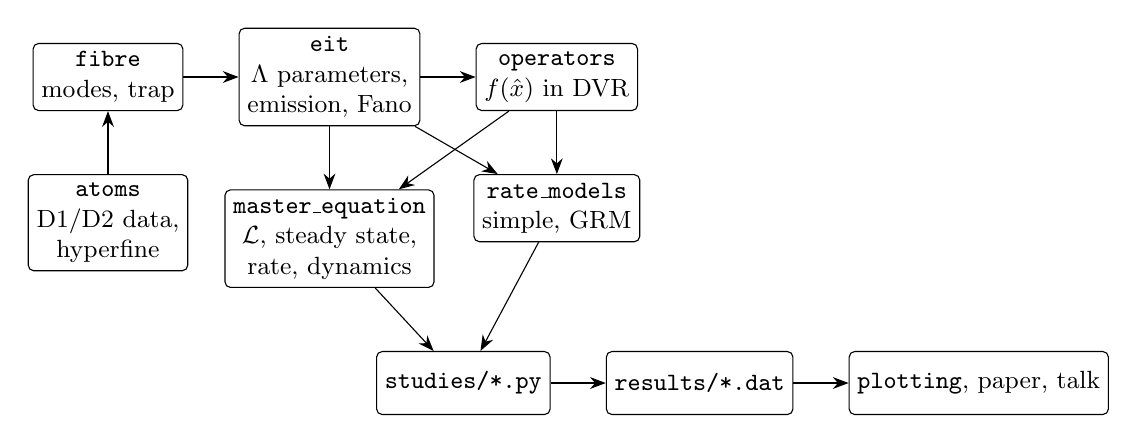
\begin{tikzpicture}[node distance=4mm and 7mm, every node/.style={font=\small},
  box/.style={draw,rounded corners=2pt,align=center,inner sep=3pt,minimum height=8mm},
  ar/.style={-{Stealth[length=2mm]}}]
\node[box] (fib) {\code{fibre}\\modes, trap};
\node[box,below=8mm of fib] (atm) {\code{atoms}\\D1/D2 data,\\hyperfine};
\node[box,right=of fib] (eit) {\code{eit}\\$\Lambda$ parameters,\\emission, Fano};
\node[box,right=of eit] (ops) {\code{operators}\\$f(\hat x)$ in DVR};
\node[box,below=8mm of eit] (me) {\code{master\_equation}\\$\mathcal L$, steady state,\\rate, dynamics};
\node[box,below=8mm of ops] (rm) {\code{rate\_models}\\simple, GRM};
\node[box,below=8mm of me,xshift=17mm] (st) {\code{studies/*.py}};
\node[box,right=of st] (res) {\code{results/*.dat}};
\node[box,right=of res] (pl) {\code{plotting}, paper, talk};
\draw[ar] (atm)--(fib); \draw[ar] (fib)--(eit); \draw[ar] (eit)--(ops);
\draw[ar] (eit)--(me); \draw[ar] (ops)--(me); \draw[ar] (ops)--(rm); \draw[ar] (eit)--(rm);
\draw[ar] (me)--(st); \draw[ar] (rm)--(st); \draw[ar] (st)--(res); \draw[ar] (res)--(pl);
\end{tikzpicture}
\caption{Module dependencies and data flow.}
\label{fig:flow}
\end{figure}

\paragraph{Units.} Inside the package all frequencies and rates are in units of the angular radial trap frequency, $\nu_r\equiv\omega_r=1$, and times in units of $1/\omega_r$. The fibre-case dictionary carries \code{om}$=\omega_r$ in rad\,s$^{-1}$. A physical rate is \code{value*fc['om']} and a physical time is \code{value/fc['om']}. With this choice the trap is always resonant with the design EIT condition (Sec.~\ref{sec:params}), and the ratio $\Gamma/\nu_r$, which is about 800 for case A, appears explicitly as the stiffness of the problem.

\paragraph{Notation.} Table~\ref{tab:notation} lists the symbols and the corresponding code names.

\begin{table}[h]
\centering\small
\caption{Symbols and code names (keys of the parameter dictionary \code{p} from \code{eit.params}).}
\label{tab:notation}
\begin{tabularx}{\textwidth}{@{}llX@{}}
\toprule
Symbol & Code & Meaning\\
\midrule
$\Gamma$ & \code{G} & D1 linewidth, $2\pi\times5.746$\,MHz\\
$\Delta$ & \code{D} & single-photon detuning of both beams (blue)\\
$\Om_c$, $\bar\Om_p$ & \code{Wc}, \code{Wp} & coupling Rabi frequency on axis; probe ``peak-equivalent'' Rabi frequency (LP$_{01}$ peak at equal power)\\
$\Gamma_n$ & \code{Gn} & width of the narrow dressed state\\
$\etap=G_{11}x_0/a$ & \code{etap} & gradient (radial) Lamb--Dicke parameter of the probe\\
$\eta_{\rm sp}=k_{795}x_0$ & \code{eta\_sp} & Lamb--Dicke parameter of a spontaneous photon\\
$s$ & \code{s} & saturation parameter $2\Om_\perp^2/\Gamma\Gamma_n$, $\Om_\perp=\etap\bar\Om_p$\\
$\epsilon$, $x_s$, $\delta_{\rm e}$ & \code{eps}, \code{xs}, \code{d2} & LP$_{01}$ admixture of the probe; trap offset (units of $x_0$); two-photon detuning error\\
$b_p$ & \code{bp} & branching ratio of $\ket e$ into $\gp$ ($b_c=1-b_p$)\\
$N$ & \code{N} & Fock-space truncation\\
\bottomrule
\end{tabularx}
\end{table}

%=====================================================================
\section{Atomic data and hyperfine structure (\code{atoms.py})}
\label{sec:atoms}
%=====================================================================
\paragraph{Data.} \code{LINES} holds, for the D1 ($5S_{1/2}\to5P_{1/2}$) and D2 ($5S_{1/2}\to5P_{3/2}$) lines, the vacuum wavelength, the decay rate $\Gamma$, the excited $J'$, the far-detuned saturation intensity for $\pi$ light and the excited hyperfine energies, all from Steck rev.~2.3.4~\cite{steck87}: D2 $\Gamma/2\pi=6.0666$\,MHz, F$'$ splittings 72.218, 156.947 and 266.650\,MHz; D1 F$'$ splitting 814.5\,MHz. For D1 the code keeps $\lambda=794.979$\,nm and $\Gamma/2\pi=5.746$\,MHz, the values behind all paper results; rev.~2.3.4 gives $5.7500(56)$\,MHz, a 0.07\% (0.7$\sigma$) difference. Only data that are measured are typed in; everything that follows from angular momentum is computed.

\paragraph{Hyperfine strengths and branching.} With $J=1/2$ and $I=3/2$, the relative strength of $F\to F'$ and the decay branching of $F'$ into $F$ are~\cite{steck87}
\begin{equation}
  S_{FF'}=(2F'+1)(2J+1)\begin{Bmatrix}J&J'&1\\F'&F&I\end{Bmatrix}^2,\qquad
  b_{F'\to F}=(2F+1)(2J'+1)\begin{Bmatrix}J&J'&1\\F'&F&I\end{Bmatrix}^2 ,
\end{equation}
with $\sum_{F'}S_{FF'}=1$ and $\sum_Fb_{F'\to F}=1$ (\code{strength}, \code{branching}; 6j symbols from \code{sympy}). For $\pi$ light and a uniform $m_F$ population the effective dipole of $F\to F'$ is $S_{FF'}$ times the far-detuned one, $\langle J\|er\|J'\rangle^2/3$, so its saturation intensity is $I_{\rm sat}/S_{FF'}$. \code{zeeman\_coupling} returns $\langle F m_F|er_q|F'm_F'\rangle/\langle J\|er\|J'\rangle$ (Wigner--Eckart with the reduced hyperfine element), which is not used yet; it is tested against Steck's sum rules and cycling-transition element so that the Zeeman model of a later stage starts from verified couplings.

\paragraph{$\Lambda$ configurations.} A closed $\Lambda$ needs an excited level coupled to both $F=1$ and $F=2$, i.e.\ $F'=1$ or 2 on either line ($F'=0$ and 3 of D2 couple to one ground level only). \code{lambda\_config(line, Fe, gp)} returns, for the probe on $F=g_p$ and the coupling beam on the other level, the branching ratio $b_p=b_{F'\to g_p}$, the line strengths $S_p$, $S_c$ of the two legs and the detunings of the other excited levels. The three-level model needs only $b_p$; $S_p$ and $S_c$ convert Rabi frequencies into powers. Table~\ref{tab:configs} lists the eight configurations.

\begin{table}[h]
\centering\small
\caption{Closed $\Lambda$ systems of $^{87}$Rb (probe on $g_p$, coupling on $g_c$). $b_p$ sets the photons per cycle $\kappa=1/b_p$.}
\label{tab:configs}
\begin{tabular}{@{}lccccccc@{}}
\toprule
Line & $F'$ & $g_p$ & $g_c$ & $b_p$ & $S_p$ & $S_c$ & other $F'$ coupled to $g_c$\\
\midrule
D1 & 1 & 1 & 2 & 1/6 & 1/6 & 1/2 & 2 (+814\,MHz)\\
D1 & 1 & 2 & 1 & 5/6 & 1/2 & 1/6 & 2 (+814\,MHz)\\
D1 & 2 & 1 & 2 & 1/2 & 5/6 & 1/2 & 1 ($-814$\,MHz)\\
D1 & 2 & 2 & 1 & 1/2 & 1/2 & 5/6 & 1 ($-814$\,MHz)\\
D2 & 1 & 1 & 2 & 5/6 & 5/12 & 1/20 & 2, 3 (+157, +424\,MHz)\\
D2 & 1 & 2 & 1 & 1/6 & 1/20 & 5/12 & 0, 2 ($-72$, +157\,MHz)\\
D2 & 2 & 1 & 2 & 1/2 & 5/12 & 1/4 & 1, 3 ($-157$, +267\,MHz)\\
D2 & 2 & 2 & 1 & 1/2 & 1/4 & 5/12 & 0, 1 ($-229$, $-157$\,MHz)\\
\bottomrule
\end{tabular}
\end{table}

\paragraph{Neighbouring excited levels (estimate).} The coupling beam, detuned by $\Delta$ to the blue of $F'$, also light-shifts $g_c$ through every other level $F''$ coupled to $g_c$, at detuning $\Delta''=\Delta-(E_{F''}-E_{F'})/\hbar$. Relative to the shift through $F'$ this is
\begin{equation}
  \frac{\delta_+^{(\rm nb)}}{\delta_+}\simeq\sum_{F''}\frac{S_{g_cF''}}{S_{g_cF'}}\frac{\Delta}{\Delta''}\qquad(\code{neighbour\_shift}),
\end{equation}
a far-off-resonance estimate that flags where the three-level model is unreliable.

\paragraph{Excited manifold (stage 2).} \code{excited\_manifold(line, Fe, gp)} lists every excited level coupled to $g_p$ or $g_c$, with its energy offset from $F'$, its branching ratio into $g_p$ and the probe and coupling amplitudes relative to the $F'$ legs, $c_p=\langle g_p\|d\|F''\rangle/\langle g_p\|d\|F'\rangle$ and likewise $c_c$, from the signed reduced hyperfine elements $\langle F\|er\|F'\rangle=(-1)^{F'+J+1+I}\sqrt{(2F'+1)(2J+1)}\{\cdots\}\langle J\|er\|J'\rangle$ (\code{reduced\_hyperfine}). This is a hyperfine-level, polarisation-averaged model: $|c|^2$ (light shifts, scattering) is exact, but the relative sign of the Raman paths through different $F''$, which decides whether they interfere constructively or destructively, depends on the polarisations and $m_F$ in reality. The code therefore computes both signs (\code{sign}$=\pm1$ on the neighbours' probe amplitudes) and treats the spread as the model uncertainty.

%=====================================================================
\section{Fibre modes and trap parameters (\code{fibre.py})}
\label{sec:fibre}
%=====================================================================
\paragraph{Modes.} The modes are those of the capillary (Marcatili--Schmeltzer) model in the weak-guidance (LP) limit~\cite{marcatili1964,snyder1983}: $\psi_{lm}=A_{lm}J_l(u_{lm}r/a)\cos l\phi$ with $J_l(u_{lm})=0$. This is the simplest model that gives the correct transverse profiles of an inhibited-coupling or bandgap core. Only the profile near the axis matters for cooling, and it is insensitive to the details of the cladding. The constants are \code{U01}$=u_{01}=2.405$ and \code{U1[m-1]}$=u_{1m}$.

\paragraph{Equal-power normalisation.} The probe amplitude is expressed through the LP$_{01}$ peak field that the same power would produce. Then $\bar\Om_p$ and the coupling Rabi frequency are compared on the same footing, and the probe power follows directly (paper Methods). From $\int|\psi|^2dA$,
\begin{equation}
  \frac{A_{1m}}{A_{01}}=\frac{\sqrt2\,|J_1(u_{01})|}{|J_2(u_{1m})|}\ (\code{amp\_ratio}),\qquad
  G_{1m}=\frac{u_{1m}}2\frac{A_{1m}}{A_{01}}\ (\code{gfac}),
\end{equation}
so that near the axis $\psi_{1m}\simeq A_{01}G_{1m}x/a$, with $G_{11}=3.49$. The code never linearises the profile: $G_{1m}$ only defines $\etap$ and the saturation parameter, while the dynamics use the full Bessel function (Sec.~\ref{sec:ops}).

\paragraph{Trap.} The LP$_{01}$ intensity $J_0^2(u_{01}r/a)$ is replaced by its best Gaussian fit, of waist $w=0.67a$ (99\% overlap). A 1D standing wave of depth $U_0$ then gives
\begin{equation}
  \omega_z=\sqrt{2U_0k_L^2/m},\qquad \omega_r=\sqrt{4U_0/mw^2},\qquad \omega_r=\omega_z\sqrt2/(k_Lw).
\end{equation}
\code{fibre\_case(a, nuz, lam\_lat, line)} fixes $\nu_z$ (300\,kHz by default) and returns the line data ($\Gamma$, $\lambda$), and $\nu_r$, $\omega_r$, $x_0=\sqrt{\hbar/2m\omega_r}$, $x_0/a$, $\eta_{\rm sp}$ and $U_0=m\omega_z^2/2k_L^2$ ($U_0/k_B=\SI{533}{\upmu K}$). Fixing $\nu_z$ rather than $U_0$ mirrors the experiment, where the axial frequency is measured. The trap is treated as harmonic. Corrections are of relative order $k_BT/U_0$ (the shift of the radial frequency is $\approx-\tfrac38k_BT/U_0$), which is why the temperature scan stops at $k_BT_r/U_0=0.1$.

\paragraph{Power.} \code{lp01\_power(fc, Om, S)} converts an LP$_{01}$-equivalent peak Rabi frequency into guided power, $P=2I_{\rm sat}(\Om/\Gamma)^2S^{-1}\pi a^2J_1^2(u_{01})$; with $S=1$ it gives the paper's 8\,nW probe at $s=1$ (case A).

\paragraph{Cases.} \code{paper\_cases(line)} returns case A ($a=15\um$, $\nu_r=7.15$\,kHz, $x_0=90$\,nm) and case B ($a=3.5\um$, $\nu_r=30.6$\,kHz, $x_0=44$\,nm). The trap does not depend on the cooling line; $\eta_{\rm sp}$ and $\Gamma$ do.

%=====================================================================
\section{$\Lambda$ parameters, emission and Fano profile (\code{eit.py})}
\label{sec:params}
%=====================================================================
\paragraph{Design conditions.} \code{params(fc, s, Delta\_G, m, eps, xs, d2, nu\_rel, bp, N)} turns physical design choices into the dimensionless parameter set used by every model. Three conditions fix the laser parameters.
\begin{enumerate}
\item \emph{Narrow resonance on the red sideband.} The weak-probe absorption~\cite{morigi2000,fleischhauer2005}
\begin{equation}
  R(\delta)=\frac{\Om_p^2\,\Gamma\,\delta^2}{\Gamma^2\delta^2+4\big[(\Delta+\delta)\delta-\Om_c^2/4\big]^2}
  \label{eq:fano}
\end{equation}
peaks where $(\Delta+\delta)\delta=\Om_c^2/4$. Requiring the peak at exactly $\delta=\nu_r$ gives $\Om_c^2=4\nu_r(\Delta+\nu_r)$. The code uses this exact form rather than the textbook approximation $\Om_c^2/4\Delta=\nu_r$, so that the comparison with the master equation is not biased by a residual detuning of order $\nu_r/\Delta$.
\item \emph{Width of the narrow state.} The coupling beam mixes $\ket e$ and $\gc$. The narrow dressed state contains the fraction $\sin^2\theta=\tfrac12\big(1-\Delta/\sqrt{\Delta^2+\Om_c^2}\big)$ of $\ket e$, hence $\Gamma_n=\Gamma\sin^2\theta$ (exact; $\simeq\Gamma\Om_c^2/4\Delta^2$). With $\Delta=3\Gamma$, $\Gamma_n\approx\nu_r/3$: the narrow line resolves the sidebands.
\item \emph{Probe strength from $s$.} With $s=2\Om_\perp^2/\Gamma\Gamma_n$ and $\Om_\perp=\etap\bar\Om_p$, $\bar\Om_p=\sqrt{s\Gamma\Gamma_n/2}/\etap$. The input $s$ is therefore the saturation of the $n=1\to0$ sideband. Because the rate ceiling is set by $\Gamma_n$ and not by $\etap$ (paper, Results), $s$ is the natural control parameter, and $\etap$ enters only through the probe power.
\end{enumerate}

\paragraph{Imperfections.}
\begin{itemize}
\item \code{eps}: amplitude of an LP$_{01}$ admixture in the probe, relative to the peak-equivalent amplitude. It restores a carrier.
\item \code{xs}: offset of the trap centre from the node, in units of $x_0$. It enters as $f(x+x_s)$ for both beams.
\item \code{d2}: two-photon detuning error $\delta_{\rm e}$, implemented as an energy offset of $\gc$.
\item \code{nu\_rel}: a mismatch between the actual and the design trap frequency, with the lasers kept at the design values. The code builds all laser parameters for the design frequency and then rescales every frequency by $r=1/\nu_{\rm rel}$, and $x_0$-dependent quantities ($\etap$, $\eta_{\rm sp}$, $x_0/a$) by $\sqrt r$. The internal unit is then the \emph{actual} trap frequency, and a study multiplies rates by $\nu_{\rm rel}\omega_r^{\rm design}$ to get physical units. This is the experimentally relevant question: what happens when the lattice depth drifts while the lasers stay put.
\end{itemize}

\paragraph{Emission pattern.} Spontaneous emission in direction $\hat{\mathbf k}$ kicks the radial coordinate by $\hbar k u_x$, with $u_x=\hat{\mathbf k}\cdot\hat{\mathbf x}$. For a dipole along $z$ the angular distribution is $\propto\sin^2\theta$ and $\langle u_x^2\rangle=2/5$~\cite{cirac1992}. The continuous distribution of $u_x$ is replaced by $K=10$ equal-weight nodes (\code{emission\_nodes}):
\begin{itemize}
\item $2\times10^6$ directions are sampled from the dipole pattern (rejection sampling, fixed seed);
\item the sorted $u_x$ values are split into $K$ equal-probability bins, and each node is the bin mean;
\item the nodes are symmetrised, $u_k\to(u_k-u_{K+1-k})/2$, so that the recoil has no net drift.
\end{itemize}
Quantile nodes reproduce the whole distribution, not only its second moment, which matters because $\eta_{\rm sp}\approx0.7$ (case A) is not small: multi-phonon recoil events are frequent, and their weight depends on the tails of $u_x$. Bin means slightly reduce the variance, giving \code{ALPHA}$=\langle u_x^2\rangle=0.397$ instead of 0.400, a 0.7\% underestimate of the recoil heating. The fixed seed makes all results reproducible to $\sim10^{-8}$, which the regression tests rely on.

\paragraph{Excited manifold.} With \code{levels} from \code{excited\_manifold}, \code{params} stores \code{p['levels']}, a list of (offset in units of $\nu_r$, $c_p$, $c_c$, $b_p$) per level; the first is the level the lasers are tuned to, and $\Delta$, $\Om_c$, $\Gamma_n$ and $s$ keep their three-level design values. Without \code{levels} the list has one entry and everything reduces to the three-level model. \code{absorption(p, delta)} is the weak-probe spectrum of the manifold: the single-excitation amplitudes on $\{g_c,e_k\}$ driven from $g_p$ solve $(H_{\rm eff}-\delta)v=-s$ with $H_{\rm eff}=-\sum_k(\Delta-\epsilon_k+i\Gamma/2)\ket{e_k}\bra{e_k}+\tfrac{\Om_c}2\sum_kc_{c,k}(\ket{e_k}\bra{g_c}+{\rm h.c.})$ and $s=\tfrac{\Om_p}2\sum_kc_{p,k}\ket{e_k}$, and $R=\Gamma\sum_k|v_k|^2$; for one level it equals the Fano profile exactly. \code{excited\_weights} gives the share of each level in the excitation on the red sideband.

\paragraph{Line.} $\Gamma$ is taken from the fibre case, so the same function serves D1 and D2; the branching ratio is passed as \code{bp} (from \code{lambda\_config}).

\paragraph{Fano function.} \code{fano(p, delta)} returns $R(\delta)/\Om_p^2$ from Eq.~\eqref{eq:fano}. It is shared by the simple model and the GRM.

%=====================================================================
\section{Operators of the radial motion (\code{operators.py})}
\label{sec:ops}
%=====================================================================
\paragraph{Why functions of $\hat x$.} The probe couples through $f_p(\hat x)=\tfrac{A_{11}}{A_{01}}J_1\big(u_{11}(\hat x+x_s)/a\big)+\epsilon J_0\big(u_{01}(\hat x+x_s)/a\big)$, the coupling through $f_c(\hat x)=J_0\big(u_{01}(\hat x+x_s)/a\big)$, and each photon through $e^{i\eta_{\rm sp}u_k(b+b^\dagger)}$. A Lamb--Dicke expansion is not acceptable, for two reasons. First, $\eta_{\rm sp}\approx0.7$ in case A. Second, the thermal states of interest extend to $x\sim\SI{1}{\upmu m}$, where the Bessel profiles are visibly non-linear. The code therefore evaluates exact functions of $\hat x$.

\paragraph{Discrete variable representation.} \code{oscillator(N)} diagonalises the truncated matrix of $b+b^\dagger$, $X=V\,{\rm diag}(w_k)\,V^\dagger$. Its eigenvalues are the zeros of the Hermite polynomial $H_N$ (scaled), i.e.\ Gauss--Hermite nodes~\cite{golub1969}. This is the discrete variable representation (DVR) of the oscillator~\cite{light1985}. A function of position is then
\begin{equation}
  f(\hat x)\simeq V\,{\rm diag}\big(f(x_0w_k)\big)\,V^\dagger \qquad(\code{function\_of\_x}),
\end{equation}
which is exact for the matrix elements between low Fock states and polynomial $f$ of sufficiently low degree, and accurate whenever the states involved lie well below the truncation edge. Two properties make the DVR the right tool here.
\begin{itemize}
\item The recoil operator $D_k=V{\rm diag}(e^{i\eta_{\rm sp}u_kw_k})V^\dagger$ is exactly unitary in the truncated space. Hence $\sum_kw_kD_k^\dagger D_k=\mathbb 1$, and the anticommutator of the dissipator can be written analytically (Sec.~\ref{sec:me}).
\item All functions of $\hat x$ commute and share one diagonalisation, which costs $O(N^3)$ once per Liouvillian.
\end{itemize}
Elements smaller than $10^{-11}$ of the largest are dropped to keep the matrices sparse.

\paragraph{Truncation edge.} Near $n\approx N$ the DVR is inaccurate: the edge eigenvalues are spurious, and the edge acts as a sink or source. The rule followed throughout is that the populated states must lie well below $N$. The edge is invisible for steady states ($N=20$ for $\langle n\rangle\lesssim0.5$, checked with 30 and 40). It is decisive for hot thermal dynamics, where recoil diffusion carries a small fraction of the atoms far up the ladder (Sec.~\ref{sec:grm}).

%=====================================================================
\section{Master equation (\code{master\_equation.py})}
\label{sec:me}
%=====================================================================
\paragraph{Model.} In the frame rotating at the two laser frequencies (Hilbert space $\{\gp,\gc,\ket e\}\otimes\{\ket n\}_{n<N}$, ordering atom $\otimes$ oscillator, index $= jN+n$),
\begin{align}
  H&=\nu_rb^\dagger b-\Delta\ket e\bra e-\delta_{\rm e}\ket{g_c}\bra{g_c}
   +\tfrac{\bar\Om_p}2\big[\ket e\bra{g_p}f_p(\hat x)+{\rm h.c.}\big]+\tfrac{\Om_c}2\big[\ket e\bra{g_c}f_c(\hat x)+{\rm h.c.}\big],\\
  \dot\rho&=\mathcal L\rho=-i[H,\rho]+\sum_{j=p,c}\sum_{k=1}^{K}\Big(C_{jk}\rho C_{jk}^\dagger-\tfrac12\{C_{jk}^\dagger C_{jk},\rho\}\Big),\quad
  C_{jk}=\sqrt{\Gamma b_jw_k}\,\ket{g_j}\bra e\otimes D_k .
\end{align}
This is the standard Lindblad form for a driven atom with recoil~\cite{cirac1992,breuer2007}. The jump operators combine the decay channel ($j$) with the discretised emission direction ($k$). Since $\sum_{jk}C^\dagger_{jk}C_{jk}=\Gamma\ket e\bra e\otimes\mathbb1$ exactly (unitarity of $D_k$), the code inserts this term directly. The approximations are those of a closed three-level $\Lambda$ system: no Zeeman structure, no other hyperfine levels, and one radial axis, with the axial motion frozen. The axial motion can be frozen because co-propagating guided beams have an axial Lamb--Dicke parameter below $10^{-3}$ (paper, Methods).

\paragraph{Several excited levels (stage 2).} With $K$ levels the atomic space is $\{\gp,\gc,\ket{e_1},\dots,\ket{e_K}\}$ and
\begin{align}
  H&\supset-\sum_k(\Delta-\epsilon_k)\ket{e_k}\bra{e_k}+\sum_k\Big[\tfrac{\bar\Om_pc_{p,k}}2\ket{e_k}\bra{g_p}f_p(\hat x)+\tfrac{\Om_cc_{c,k}}2\ket{e_k}\bra{g_c}f_c(\hat x)+{\rm h.c.}\Big],\\
  C_{jkl}&=\sqrt{\Gamma b_{kj}w_l}\,\ket{g_j}\bra{e_k}\otimes D_l .
\end{align}
Decays of different excited levels are independent: their cross terms oscillate at the hyperfine splittings ($\ge12\Gamma$) and are dropped (secular approximation). For $K=1$ the code performs the same operations as the three-level version and reproduces it to $10^{-13}$. The cost is set by the LU fill: $1.7\times10^7$ non-zeros and $\approx20$\,s for $K=4$, $N=20$ (all three SuperLU orderings tried; \code{MMD\_AT\_PLUS\_A} remains best). Studies with many solves therefore run configurations in parallel processes (\code{WORKERS}$=4$, memory-limited at $\sim1$\,GB per factorisation).

\paragraph{Vectorisation.} $\rho$ is stacked column-wise, so ${\rm vec}(A\rho B)=(B^{\rm T}\otimes A)\,{\rm vec}(\rho)$. Then
\begin{equation}
  \mathcal L=-i(\mathbb1\otimes H-H^{\rm T}\otimes\mathbb1)+\sum_{jk}C_{jk}^*\otimes C_{jk}-\tfrac12\big(\mathbb1\otimes C^\dagger C+(C^\dagger C)^{\rm T}\otimes\mathbb1\big),
\end{equation}
a sparse matrix of dimension $(3N)^2$ (3600 for $N=20$, $3.2\times10^4$ for $N=60$).

\paragraph{Steady state.} $\mathcal L$ is singular, with one zero eigenvalue for a unique steady state. The first row of $\mathcal L$ (the equation for $\dot\rho_{00}$) is replaced by the trace condition $\sum_i\rho_{ii}=1$. No information is lost, because trace preservation makes the rows for the diagonal elements linearly dependent. The modified matrix is factorised once by sparse LU (SuperLU~\cite{li2005}). The column ordering \code{MMD\_AT\_PLUS\_A} is about $4\times$ faster than the default for this structure. The result is Hermitised to remove round-off.

\paragraph{Cooling rate.} The rate is defined through the \emph{integrated} relaxation of $\langle n\rangle$ after preparing $\rho_0=\ket{g_p,1}\bra{g_p,1}$:
\begin{equation}
  W^{-1}=\int_0^\infty\frac{\langle n\rangle(t)-n_{\rm ss}}{n_0-n_{\rm ss}}\,dt
        =-\frac{{\rm Tr}\big[\hat n\,\mathcal L^{-1}(\rho_0-\rho_{\rm ss})\big]}{n_0-n_{\rm ss}} .
\end{equation}
Because ${\rm Tr}(\rho_0-\rho_{\rm ss})=0$, the right-hand side lies in the range of $\mathcal L$. The solution with zero trace is obtained with the same factorisation by setting the first element of the source to zero (\code{relax\_rate}): one extra triangular solve, with no time integration. The slowest non-zero eigenvalue of $\mathcal L$ is deliberately \emph{not} used. Saturated high-$n$ states cool linearly in time, not exponentially, so the spectrum contains slow modes localised near the truncation edge, and these drift with $N$. The integrated time is dominated by the populated low-$n$ states and agrees with the $1/e$ time for exponential relaxation.

\paragraph{Time evolution.} The problem is stiff: optical rates $\sim\Gamma=800\nu_r$ coexist with cooling rates $\sim10^{-1}\nu_r$. \code{evolve} uses the second-order backward differentiation formula (BDF2), started with one implicit Euler step:
\begin{equation}
  (3-2h\mathcal L)\,y_{n+1}=4y_n-y_{n-1}.
\end{equation}
BDF2 is A- and L-stable~\cite{hairer1996}. The fast optical transients are damped rather than resolved, which is equivalent to adiabatically following the internal state, while the motional dynamics are integrated to second order. With $h=0.02/\nu_r$ one LU factorisation serves the whole run, and the ME relaxation of Fig.~5a (case A, $N=30$) takes about 6\,min.

\paragraph{Phonon drift from a Fock state.} \code{fock\_drift} prepares $\ket{g_p,n_0}$, propagates with implicit Euler ($h=0.05$), and measures $d\langle n\rangle/dt$ between $t=5$ and $20/\nu_r$, after the internal transient ($\sim1/\Gamma_n$) has settled. This is the observable used to calibrate and test the GRM. A truncation $N\approx2n_0$ suffices: for $n_0=20$, $N=45$ and $N=60$ differ by 0.3\%.

%=====================================================================
\section{Rate models (\code{rate\_models.py})}
\label{sec:rates}
%=====================================================================
\subsection{Simple model}
\label{sec:simple}
\code{simple(p, photons)} is the sideband rate equation of Morigi \emph{et al.}~\cite{morigi2000}, with three fibre-specific additions (paper, Methods). The sideband rates are $A_\mp=\Om_\perp^2R(\pm\nu_r+\delta_{\rm e})/\Om_p^2$, and
\begin{equation}
  W=A_-(1-h)-A_+(1+h),\qquad n_{\rm ss}=\frac{A_+(1+h)}{W},\qquad h=\kappa\,\alpha\eta_{\rm sp}^2 .
\end{equation}
\begin{itemize}
\item[(i)] \emph{Photons per cycle,} $\kappa$ (\code{photons}). After a decay into $\gc$ the coupling beam re-excites the atom, so a cycle ends in $\gp$ after $\kappa=1/b_p$ photons on average. The ME includes this automatically; a rate model must add it by hand. With $\kappa=1$ the model underestimates $n_{\rm ss}$ by 40\% (case A).
\item[(ii)] \emph{Recoil per photon,} $\alpha\eta_{\rm sp}^2$, where $\alpha=$\code{ALPHA}. This is exact for the mean energy at any $\eta_{\rm sp}$, since the recoil energy is $E_{\rm rec}=\hbar\omega_r\eta_{\rm sp}^2$ per unit $u_x^2$~\cite{leibfried2003}.
\item[(iii)] \emph{Saturation of the red sideband only,} $A_-\to A_-/(1+s)$. Only $A_-$ is resonant with the narrow line; $A_+$ is off-resonant and does not saturate.
\end{itemize}
\code{unified(p)} is the simple model's estimate of the best rate with an LP$_{01}$ admixture. The carrier $\epsilon\bar\Om_p$ must stay below $\Om_c/3$~\cite{morigi2003}, which caps $s$ at $8(\Delta/3\Gamma)^2(\etap/\epsilon)^2$. The function returns $(1-2\alpha\eta_{\rm sp}^2)\tfrac{\Gamma_n}2\tfrac{s}{1+s}$ with $s=\min(1,\text{cap})$. It is the curve the ME impurity scan is compared with.

\subsection{Generalised rate model}
\label{sec:grm}
\paragraph{Purpose.} Cooling from \SI{10}{\upmu K} involves $\langle n\rangle\approx30$ (A), and the temperature scan up to $\langle n\rangle\approx155$. The ME would need $N\gtrsim500$ and $(3N)^2\sim10^6$ unknowns with a dense fill-in, which is out of reach. The GRM keeps only the populations $p_n$ of $\ket{g_p,n}$ and treats the internal dynamics as instantaneous. This is justified because $\Gamma_n\gg W$.

\paragraph{Construction} (\code{grm\_matrix}). Three ingredients, all evaluated with the exact DVR operators:
\begin{enumerate}
\item \emph{Absorption} $n\to m$ at rate
\begin{equation}
  K_{mn}=\frac{\bar\Om_p^2\,|\bra mf_p(\hat x)\ket n|^2\,R\big((n-m)\nu_r+\delta_{\rm e}\big)/\Om_p^2}{1+c_{\rm sat}s_n},\qquad
  s_n=\frac{2\bar\Om_p^2|\bra{n-1}f_p\ket n|^2}{\Gamma\Gamma_n}.
\end{equation}
The Fano profile selects the energy-conserving transitions; the full Bessel profile includes the higher-order odd sidebands ($\Delta n=\pm3,\dots$); $s_n$ is the saturation of the resonant sideband out of $n$ and divides all transitions out of $n$.
\item \emph{Recoil kernel of one photon,} $P_{n'm}=\sum_kw_k|\bra{n'}D_k\ket m|^2$, normalised column-wise to remove the probability lost at the truncation edge.
\item \emph{Redistribution per cycle.} A decay into $\gp$ ends the cycle; a decay into $\gc$ is followed by re-excitation by the coupling beam and another photon. Summing the geometric series gives $T=b_pP(\mathbb1-b_cP)^{-1}$. The re-excitation is assumed not to change $n$: the LP$_{01}$ coupling field is flat at the node, and its curvature enters only at second order.
\end{enumerate}
The generator is $Q=TK-{\rm diag}\big(\sum_mK_{mn}\big)$ with $\dot{\bm p}=Q\bm p$. Dynamics use $e^{Q\Delta t}$ (dense \code{scipy.linalg.expm}) applied repeatedly on a uniform grid, and the steady state is the eigenvector of the eigenvalue closest to zero (\code{grm\_steady\_state}). \code{thermal(nbar, N)} gives the truncated Bose distribution used as initial state.

\paragraph{Several excited levels.} Both rate models take the sideband rates from \code{absorption}, so they include the light shifts and interference of the whole manifold. In the GRM the branching ratio of a cycle is that of the excited mixture reached on the red sideband, $b_p=\sum_kw_kb_{kp}$ with $w_k$ from \code{excited\_weights}. $c_{\rm sat}$ has not been recalibrated for $K>1$.

\paragraph{What the GRM misses.} The GRM is a perturbative picture in which each sideband is an incoherent rate. At $s\gtrsim0.1$ the effective Raman coupling $\Om_R=\Om_c\Om_\perp/2\Delta$ between $\ket{g_p,n}$ and $\ket{g_c,n\mp1}$ becomes comparable to $\Gamma_n$, with $\Om_R^2=s\Gamma_n^2/2$. The narrow resonance then splits, and coherences between $\gp$ and $\gc$ build up. The plain saturation factor ($c_{\rm sat}=1$) overestimates the saturated phonon-removal rate by a factor of 2--2.5. The constant $c_{\rm sat}$ absorbs this to leading order.

\subsection{Calibration and validity of the GRM}
\label{sec:calib}
\paragraph{Calibration} (\code{studies/calibration.py drift}). $c_{\rm sat}$ is fitted to the ME drift $d\langle n\rangle/dt$ from Fock states $n_0=1,3,6,10,15$, at $s=0.2$ and 1, for both cases. Minimising the rms logarithmic error gives \code{CSAT}$=2.25$ (17\% rms). The fit uses the drift because it is the quantity that controls thermal dynamics, and Fock states because they probe each rung of the ladder separately. As a check, the calibrated GRM reproduces the ME relaxation from $\langle n\rangle=2$ (case A, $s=0.2$) within 8\% (paper Fig.~5a).

\paragraph{Extrapolation} (\code{studies/temperature.py drift}). At $s=1$ the GRM gives 0.75 and 0.42 of the ME drift for $n_0=20$ and 30 (case A), and 0.83 and 0.56 (case B). The ME drift keeps growing with $n_0$, while the calibrated GRM saturates at $\approx1.9$ (A) and $12.5$ (B) phonons per ms. Beyond its calibration range the GRM is therefore \emph{conservative}: cooling times of hot states are upper bounds.

\paragraph{Truncation of the GRM.} Recoil changes $n$ by $\approx\eta_{\rm sp}u\sqrt{2n}$ per photon. A hot atom therefore diffuses in energy over a cooling time by an amount comparable to its own energy, and a small fraction of the population climbs far up the ladder. With $N$ too small, the truncation edge acts as an artificial sink (with $N=300$ the drift jumps from $-1.9$ to $-26$ phonons/ms near the top of the ladder), and $\langle n\rangle$ at late times is underestimated. In case A from \SI{10}{\upmu K}, $N=300$ gives $\langle n_x\rangle=0.24$ after 150\,ms, against 1.15 ($N=800$) and 1.45 ($N=1600$). The ground-state population is stable to 0.3\%. The code uses $N$ up to the trap depth, $U_0/\hbar\omega_r=1552$ (A) and 362 (B), i.e.\ $N=1600$ and 400. This is the largest physically meaningful ladder in the harmonic model.

%=====================================================================
\section{Studies}
\label{sec:studies}
%=====================================================================
Each script in \code{studies/} reproduces one group of results. Table~\ref{tab:studies} lists them; \code{run\_all.py} runs them all (about 55\,min). \code{\_common.py} holds the paths, the two cases and $N=20$ for ME steady states.

\begin{table}[h]
\centering\small
\caption{Study scripts; figure and table numbers refer to the paper. ``ME'' = master equation, ``SM'' = simple model, ``GRM'' = generalised rate model.}
\label{tab:studies}
\begin{tabularx}{\textwidth}{@{}lXll@{}}
\toprule
Script (sub-study) & What is varied, and why & Model & Output / paper item\\
\midrule
\code{saturation} & $s=10^{-2}$--10: rate and $n_{\rm ss}$, SM with $\kappa=1$ and 2; finds where the SM fails & ME, SM & \code{sat\_\{A,B\}}, Fig.~3\\
\code{robustness carrier} & $\epsilon$ and $x_s$ at the $s$ that maximises $W$: tolerance to mode impurity and offset & ME & \code{carrier\_A}, Fig.~4a\\
\code{robustness twophoton} & $\delta_{\rm e}$ at $s=0.2$, with and without $\epsilon=0.05$: node versus carrier & ME, SM & \code{twophoton\_A}, Fig.~4b\\
\code{robustness mismatch} & $\nu_r/\nu_r^{\rm design}=0.6$--1.6, lasers fixed: lattice-depth drift & ME, SM & \code{mismatch\_\{A,B\}}, Fig.~4c\\
\code{calibration steady} & $n_{\rm ss}$ of GRM ($c_{\rm sat}=1$) versus ME & ME, GRM & \code{grmcheck}\\
\code{calibration drift} & Fock-state drift, fit of $c_{\rm sat}$ & ME, GRM & \code{drift\_calib}, Tab.~3\\
\code{dynamics relaxation} & from $\langle n\rangle=2$ (A, $s=0.2$): validates the GRM in time & ME, GRM, SM & \code{dyn\_A}, Fig.~5a\\
\code{dynamics capture} & from \SI{10}{\upmu K}, four protocols (incl.\ staged $\Delta$, LP$_{12}$) & GRM & \code{capture\_\{A,B\}}, Fig.~5b,c\\
\code{temperature scan} & $k_BT_r/U_0=10^{-3}$--$10^{-1}$, 20 log steps, $s=1$ & GRM & \code{temperature}, \code{temptrace}, Fig.~6\\
\code{temperature drift} & ME drift at $n_0=20,30$: GRM extrapolation & ME, GRM & \code{drift\_hi}\\
\code{lines effective} & every closed $\Lambda$ (D1/D2, $F'$, $g_p$), $s=0.01$--10: rate, $n_{\rm ss}$, powers, neighbour shift & ME, SM & \code{lines}, \code{lines\_scan}\\
\code{lines multilevel} & every $\Lambda$ with all excited levels, $\Delta=3\Gamma$, $s=1$, both interference signs; lasers as designed and with $\delta_{\rm e}$ re-optimised & ME, SM & \code{lines\_ml}\\
\code{lines delta} & cooling configurations ($b_p\ge1/2$) versus $\Delta/\Gamma=1$--12, $\delta_{\rm e}$ re-optimised & ME & \code{lines\_delta}\\
\code{report\_scaling} & analytic scaling for the background report (independent of \code{eitsim}) & analytic & \code{results/report/}\\
\bottomrule
\end{tabularx}
\end{table}

Three study-level choices deserve a comment.
\begin{itemize}
\item \emph{Maximum rate under impurity.} For each $\epsilon$ or $x_s$, the carrier study scans $s$ and keeps the best $W$, because an experiment would re-optimise the probe power. A trap offset is converted to an equivalent admixture, $\epsilon_{\rm eff}=\etap x_s/x_0$, which follows from expanding $J_1$ around $x_s$.
\item \emph{Metrics of the temperature scan.} The initial occupation is Bose--Einstein, $\bar n_0=1/(e^{\hbar\omega_r/k_BT}-1)$, not the classical $k_BT/\hbar\omega_r$, because the cold end has $\bar n_0<1$. Three metrics are reported: the $1/e$ time of the excess $\langle n\rangle-n_{\rm ss}$, the time to reach $P_0\ge0.9$, and the initial phonon-removal rate $-\sum_n n\,(Q\bm p_0)_n$. The ground-state criterion is used because it is insensitive to the sparse hot tail that dominates $\langle n\rangle$ at late times.
\item \emph{Re-optimised two-photon detuning (stage 2).} The other excited levels light-shift $g_c$ and move the narrow resonance off the red sideband; an experiment compensates this by retuning the Raman detuning. \code{optimise\_d2} locates the narrow resonance as the strongest interior maximum of the multi-level absorption within $\pm10\nu_r$ (cheap), then refines $\delta_{\rm e}$ with three or four ME solves (parabola). The selection is restricted to $n_{\rm ss}<0.2$, because the relaxation rate from $\ket{g_p,1}$ is ill-defined when $n_{\rm ss}$ is not small (it can even become negative); points above are flagged in the output. When the neighbours wash the narrow resonance out (D2 $F'=1$ at large $\Delta$), no peak exists and cooling fails.
\item \emph{Capture protocols.} The staged protocol starts with $\Delta=\Gamma$, which gives a broader narrow line and faster capture of hot atoms, and switches to $\Delta=3\Gamma$ for a lower floor. LP$_{12}$ is included to show that the mode order affects only the probe power.
\end{itemize}

%=====================================================================
\section{Figures, tests and reproducibility}
%=====================================================================
\paragraph{Plotting.} \code{plotting/style.py} fixes the Nature figure style (Arial 7\,pt, 183\,mm width, Okabe--Ito colours). \code{make\_figures.py} reads only \code{results/} and writes \code{paper/manuscript/figures/}. Rule: no text may overlap data; legends are placed outside the axes or in regions kept empty by fixed axis limits.

\paragraph{Regression tests} (\code{tests/test\_regression.py}, $\sim30$\,s, run before every commit to \code{simulation/}). They check:
\begin{itemize}
\item the mode constants ($G_{11}$, $A_{11}/A_{01}$, $\langle u_x^2\rangle$) and the trap parameters of both cases;
\item that the ME reproduces a stored point of \code{sat\_A} to $10^{-6}$ and the SM points of \code{sat\_B} to $10^{-9}$;
\item the GRM steady state against \code{grmcheck};
\item the initial states and ground-state outcome of the temperature scan, one recomputed scan point, the high-$n$ GRM drift and the threshold helper;
\item the atomic data: $S_{FF'}$ against Steck's Table~8, the sum rules for $S_{FF'}$, $b_{F'\to F}$ and the Zeeman couplings, the D2 cycling element, the allowed $\Lambda$ configurations;
\item that the D1 fibre case is unchanged by the line parameter, and that the D1 rows of the line study reproduce \code{sat\_B};
\item the stage-2 model: manifold amplitudes against $S_{FF'}$, the one-level and decoupled-level limits of \code{absorption}, far neighbours reproducing the three-level ME, and one recomputed point of \code{lines\_ml}.
\end{itemize}
Any change in the physics, the quadrature or the numerics shows up as a failure, which is then resolved by rerunning the affected study, never by editing results.

\paragraph{Determinism and convergence.} The only random element is the emission quadrature, which uses a fixed seed. Table~\ref{tab:conv} summarises the convergence checks behind the numerical choices.

\begin{table}[h]
\centering\small
\caption{Numerical parameters and their checks.}
\label{tab:conv}
\begin{tabularx}{\textwidth}{@{}lXX@{}}
\toprule
Parameter & Value & Check\\
\midrule
ME truncation, steady state & $N=20$ & unchanged with $N=30$, 40 for $\langle n\rangle\lesssim0.5$\\
ME truncation, dynamics & $N=30$ from $\langle n\rangle=2$ & population at $n>25$ negligible\\
ME truncation, Fock drift & $N=45$ ($n_0=20$), 60 ($n_0=30$) & $N=60$ changes $n_0=20$ by 0.3\%\\
GRM truncation & $N=1600$ (A), 400 (B) & trap depth (physical limit); $P_0$ stable to 0.3\%; $\langle n\rangle$ at late times changes by 20\% between $N=800$ and 1600\\
Emission nodes & $K=10$ & $\langle u_x^2\rangle=0.397$ (exact 0.4)\\
BDF2 step & $h=0.02/\nu_r$ & second order; L-stable for the optical modes\\
Fock-drift window & $t=5$--$20/\nu_r$ & after the internal transient $\sim1/\Gamma_n$\\
\bottomrule
\end{tabularx}
\end{table}

%=====================================================================
\section{Limits of the model and where to extend it}
%=====================================================================
The model is an ideal closed $\Lambda$ system with one radial axis. Each limitation below has a natural place in the code.
\begin{itemize}
\item \emph{Atomic structure.} The excited hyperfine manifold is included (stage 2), but without Zeeman structure: the relative sign of Raman paths through different $F'$ is bracketed, not computed. Zeeman sublevels, polarisation-resolved couplings (and the dark states they create), magnetic-field remixing and the excited-state light shift of the lattice (tensor part for $5P_{3/2}$) require the Zeeman-resolved model of the next stage; \code{zeeman\_coupling} already provides its couplings. For the full Zeeman problem, adiabatic elimination of the excited states (effective-operator formalism~\cite{reiter2012}) keeps the problem tractable.
\item \emph{Second radial axis.} The radial motion is separable in the harmonic approximation, but the LP$_{11}$ lobe addresses only $x$. Cooling of $y$ needs the orthogonal lobe or trap anisotropy; this means two oscillators, or alternating stages in the GRM.
\item \emph{Anharmonic trap and loss.} Above $k_BT_r/U_0\approx0.1$, a Gaussian radial potential and an absorbing boundary at $U_0$ are needed. Both fit naturally into the GRM, through an energy-dependent $\omega_r(n)$ and an absorbing state.
\item \emph{Collective effects} (reabsorption, probe depletion) are estimated analytically in the background report and not simulated.
\end{itemize}

\bibliographystyle{unsrtnat}
\bibliography{refs}

\end{document}
